\documentclass[a4paper,titlepage,11pt,floatssmall]{mwrep}
\usepackage[left=2.5cm,right=2.5cm,top=2.5cm,bottom=2.5cm]{geometry}
\usepackage[OT1]{fontenc}
\usepackage{polski}
\usepackage[utf8]{inputenc}
\usepackage{amsmath}
\usepackage{amssymb}
\usepackage{graphicx}
\usepackage{mathrsfs}
\usepackage{rotating}
\usepackage{pgfplots}
\usetikzlibrary{pgfplots.groupplots}

\usepackage{siunitx}

\usepackage{float}
\definecolor{szary}{rgb}{0.95,0.95,0.95}
\sisetup{detect-weight,exponent-product=\cdot,output-decimal-marker={,},per-mode=symbol,binary-units=true,range-phrase={-},range-units=single}

\SendSettingsToPgf
\title{\bf Sprawozdanie z laboratorium nr 5\\ Formatowanie ciągów znaków przy użyciu mikrokontrolera z rodziny MSP430 z zastosowanie transmisji szeregowej  \vskip 0.1cm}
\author{Jakub Sikora \and Konrad Winnicki \and Marcin Dolicher}
\date{\today}
\pgfplotsset{compat=1.15}	
\begin{document}


\makeatletter
\renewcommand{\maketitle}{\begin{titlepage}
		\begin{center}{\LARGE {\bf
					Wydział Elektroniki i Technik Informacyjnych}}\\
			\vspace{0.4cm}
			{\LARGE {\bf Politechnika Warszawska}}\\
			\vspace{0.3cm}
		\end{center}
		\vspace{5cm}
		\begin{center}
			{\bf \LARGE Technika Mikroprocesorowa \vskip 0.1cm}
		\end{center}
		\vspace{1cm}
		\begin{center}
			{\bf \LARGE \@title}
		\end{center}
		\vspace{2cm}
		\begin{center}
			{\bf \Large \@author \par}
		\end{center}
		\vspace*{\stretch{6}}
		\begin{center}
			\bf{\large{Warszawa, \@date\vskip 0.1cm}}
		\end{center}
	\end{titlepage}
	}
\makeatother
\maketitle

\tableofcontents


\chapter{Zadanie laboratoryjne}
\section{Polecenie}
Korzystając z pakietu z mikrokontrolerem MSP430 oraz innych modułów systemu SML-3 należy zrealizować system o funkcjonalności jak w ćwiczeniu 4, 
z zastąpieniem przycisków i wyświetlacza terminalem znakowym (klawiatura + ekran PC) dołączonym przez port RS-232.

Wybrane zadanie dodatkowe:
16.   korygowanie linii tekstu zakończonych znakiem CR przez usuwanie powtórzonych znaków i zbędnych spacji oraz konwersję wielkich liter, np.:
"ALA ma Kooota  , 1123" -> "Ala ma kota, 123"

UWAGI
- proszę przemyśleć funkcje systemu (i ewentualnie wzbogacić interakcję) oraz sposób jego uruchamiania;
- w razie potrzeby proszę sformułować dodatkowe założenia zmieniające funkcjonalność z uwzględnieniem specyfiki transmisji szeregowej;
- nadawanie i odbieranie danych należy realizować z największą dostępną szybkością, buforowaniem programowym i z użyciem przerwań;
- w przypadku pomiarów należy oszacować użyteczny zakres i dokładność. 

Realizacja zadania z puli dodatkowej umożliwia uzyskanie do 2 dodatkowych punktów.
Użycie w rozwiązaniu sterownika DMA umożliwia uzyskanie do 2 dodatkowych punktów.
\section{Szczegółowe uwagi}
Należy przemyśleć funkcje systemu (i ewentualnie wzbogacić interakcję) oraz sposób jego uruchamiania. W razie potrzeby proszę sformułować dodatkowe założenia zmieniające funkcjonalność z uwzględnieniem specyfiki transmisji szeregowej. Nadawanie i odbieranie danych należy realizować z największą dostępną szybkością, buforowaniem programowym i z użyciem przerwań;
W przypadku pomiarów należy oszacować użyteczny zakres i dokładność. 

Realizacja zadania z puli dodatkowej umożliwia uzyskanie do 2 dodatkowych punktów.
Użycie w rozwiązaniu sterownika DMA umożliwia uzyskanie do 2 dodatkowych punktów.


\chapter{Projekt urządzenia}
\section{Komponenty sprzętowe}
Dzięki strukturze mikrokontrolera MSP430F16x podłączenie urządzeń peryferyjnych nie było skomplikowanym zadaniem, jednak wymagało uwagi aby odpowiednio połączyć ze sobą porty na PC (Tx i Rx) i mikrokontrolerze odpowiadające za komunikację. Zgodnie z rysunkiem, bity transmitowane z rejestru nadawczego Tx mikrokontrolera powinny być odbierane w rejestrze odbiorczym Rx komputera PC i analogicznie rejestr Tx komputera PC powinnien być połączony z rejestrem Rx mikrokontrolera.

\begin{figure}[H]
\centering
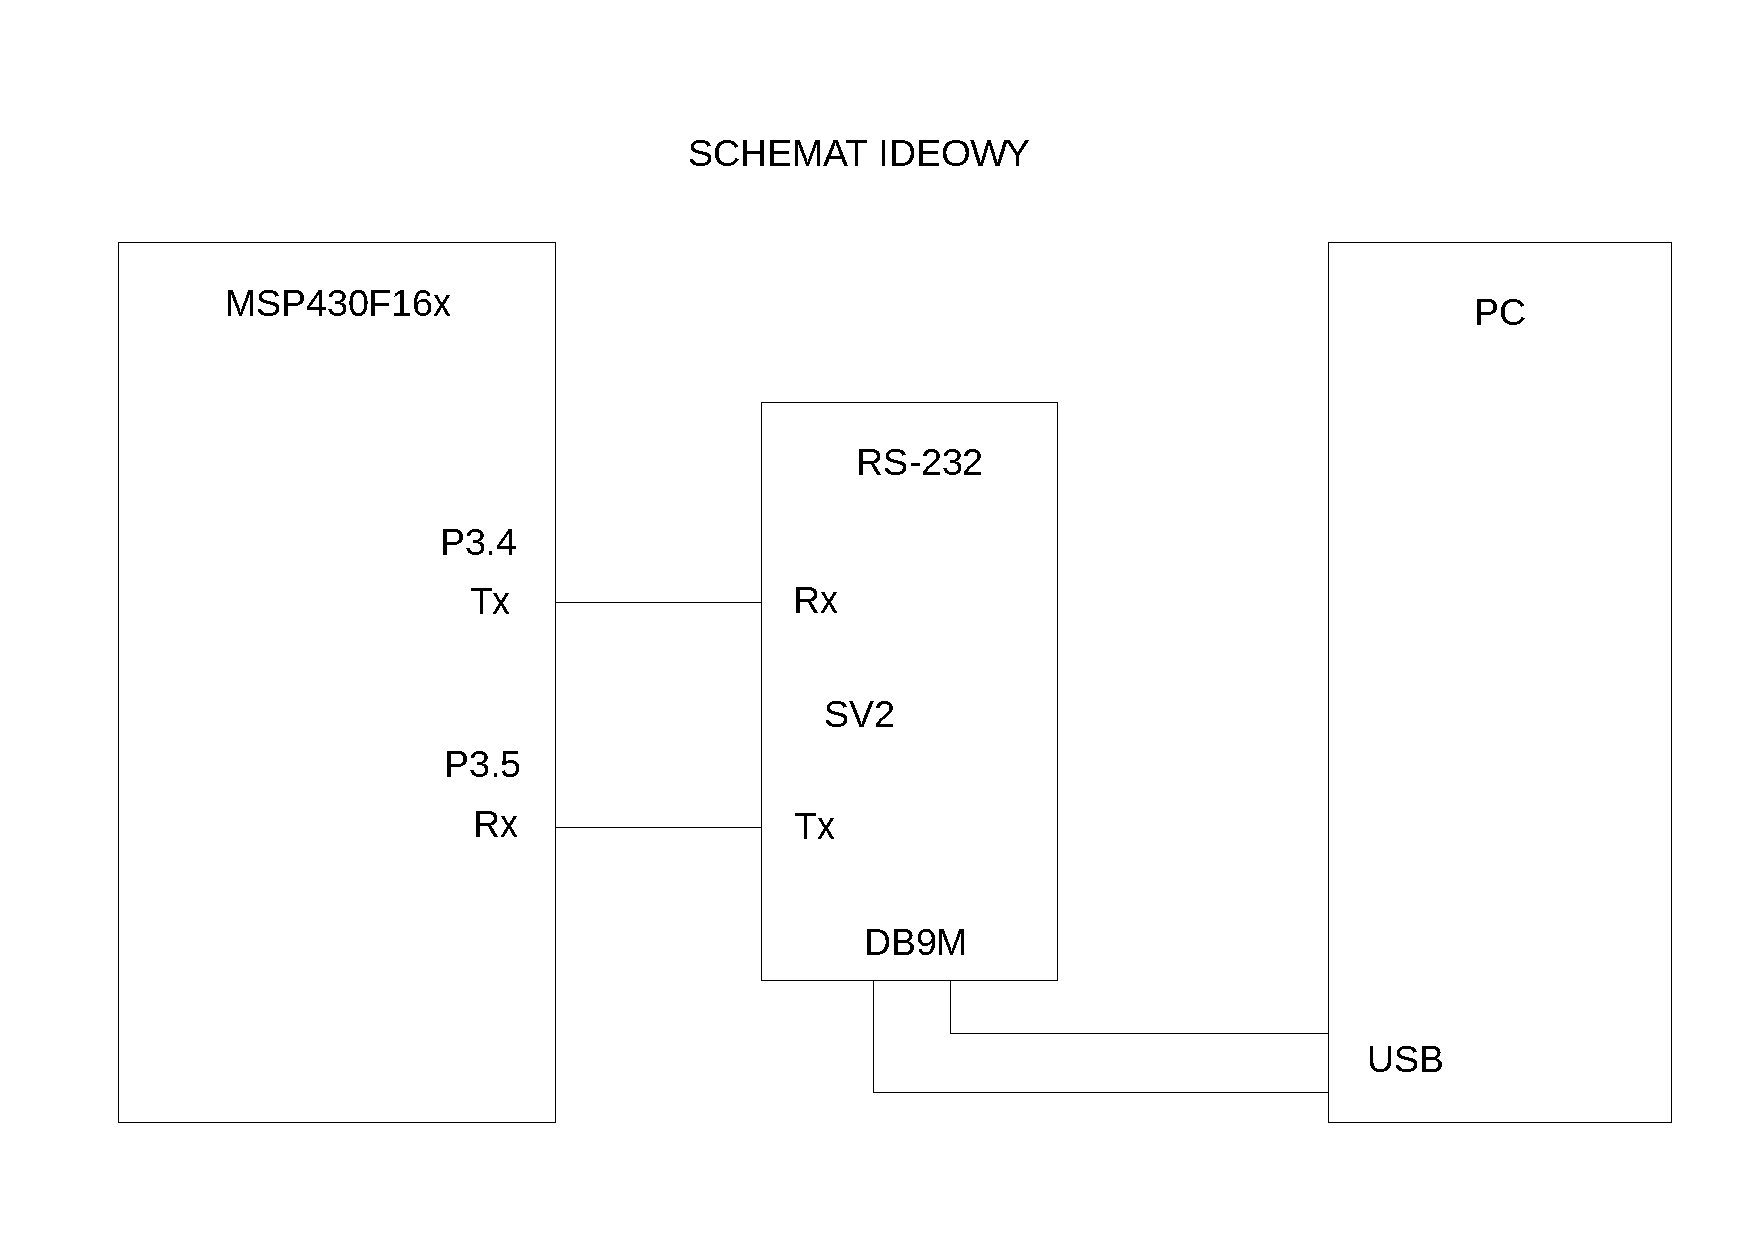
\includegraphics[width=\textwidth]{img/Ideowy.pdf}
\caption{Schemat ideowy urządzenia realizującego zadanie projektowe}
\end{figure}

Do portów P3.4 – Tx, P3.5 – Rx w mikrokontrolerze podłączyliśmy sygnały Rx i Tx z linii SV2 pochodzącej z modułu łącza szeregowego RS232. Moduł ten łączy się z komputerem za pomocą złącza DB9M, które łaczy się z układem MAX238 który spełnia rolę sterownika transmisji który ustala poziomy napięć na szynach transmisyjnych na zgodne ze standardem RS-232.

\newpage
\section{Opis oprogramowania}
Kod programu napisaliśmy w języku C, ale w porównaniu do zadań z poprzednich laboratoriów warstwa programowa była zdecydowanie bardziej rozbudowana. Po raz pierwszy zdecydowaliśmy się na podział kodu na kilka plików aby uczynić projekt czytelniejszym. Użycie języka C zamiast assemblera pozwoliło na lepsze uporządkowanie funkcjonalności i zadań do wykonania w naszym programie. Kod stał się bardziej przejrzysty i zrozumiały.\\

\subsubsection{Bufory cykliczne i warstwa sprzętowa}
\indent{}Zgodnie z zaleceniem, zdecydowaliśmy się na podział oprogramowania na warstwę sprzętową i warstwę aplikacyjną. Warstwa sprzętowa zajmowała się obsługą przerwań, wysyłaniem bajtów do komputera i ich odbieraniem. Zadaniem warstwy aplikacyjnej było przetwarzanie zagregowanych wcześniej ciągów bajtów zgodnie z poleceniem. Komunikacja pomiędzy dwoma warstwami odbywała się za pomocą buforów cyklicznych. 

\begin{figure}[H]
\centering
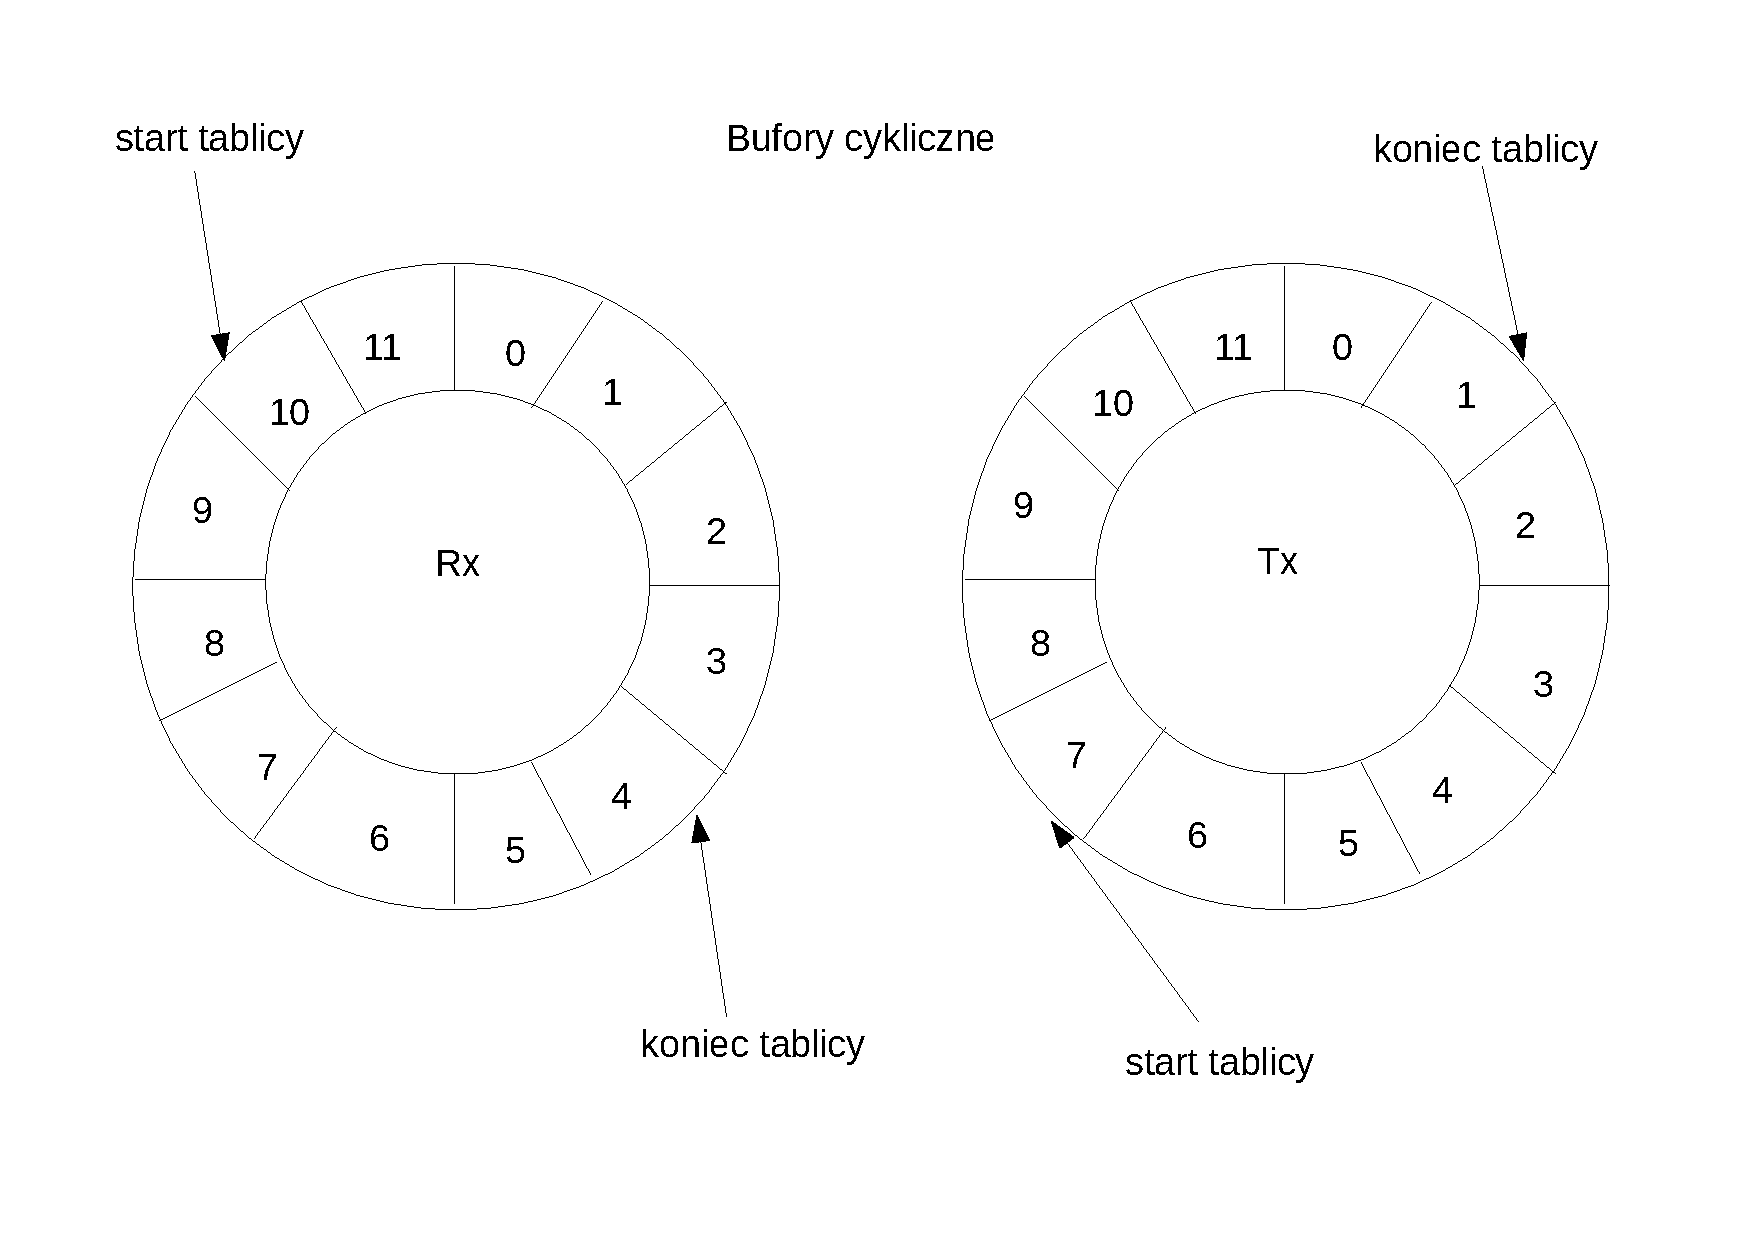
\includegraphics[width=\textwidth]{img/bufory_obrazek.pdf}
\caption{Zasada działania buforów cyklicznych}
\end{figure}

Idea bufora cyklicznego polega na dwóch znacznikach - zapisu i odczytu, wskazujące kolejno na pozycję do zapisu i odczytu pojedynczej danej z tablicy bufora o ustalonym rozmiarze.
Dane możliwe do odczytu znajdują się pomiędzy znacznikiem odczytu, a znacznikiem zapisu. 
Możliwa jest sytuacja gdy pozycja znacznika zapisu jest poniżej pozycji znacznika odczytu, taka sytuacja oznacza, że nastąpił cykl bufora – znacznik zapisu osiągnął koniec tablicy bufora i przeskoczył na początek tejże tablicy. Analogiczna sytuacja występuje w przypadku znacznika odczytu.

\newpage

Opis implementacji:\\
	Biblioteka bufora cyklicznego składa się z plików:\\
	\indent{}data\_{}buffer.h – plik nagłówkowy\\
	\indent{}data\_{}buffer.c – kody źródłowe bufora\\
	\medskip
Biblioteka w swym pliku nagłówkowym dostarcza metodę tworzenia bufora cyklicznego o podanym rozmiarze oraz nazwie:\\
	\indent{}\#{}define RX\_{}2BUFFER\_{}INDEX 100 /* rozmiar tworzonego bufora<=255 */\\
\indent{} DATA\_{}BUFFER\_{}CREATE(rx\_{}data\_{}buffer\_{}tab, RX\_{}BUFFER\_{}INDEX, rx\_{}data\_{}buffer) /* stworzenie bufora o podanych parametrach */\\

Bufory są osiągalne przy użyciu funkcji:\\
	data\_{}buffer\_{}write – zapis danej do bufora\\
	data\_{}buffer\_{}read – odczyt danej z bufora\\
	data\_{}buffer\_{}number – ilość danych w buforze\\

Dostępne są również makra pozwalające ustalić stan bufora:\\
	DATA\_{}BUFFER\_{}READY\_{}TO\_{}READ – czy bufor jest gotowy do odczytu\\
	DATA\_{}BUFFER\_{}READY\_{}TO\_{}WRITE – czy bufor jest gotowy do zapisu\\

W momencie odebrania bajtu, bajt jest przesyłany z rejestru Rx do odpowiadającego bufora cyklicznego. W momencie gdy aplikacja potrzebuje pobrać pobrać dane, pobiera je z bufora cyklicznego a nie z rejestru Rx. To rozwiązanie jest uniwersalne i może być stosowane niezależnie od aplikacji. Obsługa rejestru nadawaczego Tx odbywa się w analogiczny sposób.

\subsubsection{Warstwa aplikacja}
Zadaniem warstwy aplikacyjnej jest sformatowanie tekstu poprzez: \\
	\indent{}- usunięcie powtarzających się znaków
usunięcie nadmiarowych spacji\\
	\indent{}- spacja pomiędzy wyrazami oraz po przecinku i kropce
 korektę małych i wielkich liter \\
\indent{}- tak aby wielka litera znajdowała się na początku każdego zdania\\
Brak rozpoznawania nazw własnych przez co po sformatowaniu rozpoczynają się one małą literą.\medskip

Implementacja aplikacji: \\
	Biblioteka aplikacji składa się z plików:\\
	\indent{}format.h – deklaracje funkcji formatujących\\
	\indent{}format.c – implementacje funkcji formatujących\\
	\medskip
W skład aplikacji wchodzą funkcje:\\
	\indent{}toLowCases	- konwersja tekstu na małe litery\\
	\indent{}formatCapitalLetter – wielkie litery na początku zdań\\
	\indent{}formatRepeatedLetters – usunięcie powtarzających się znaków\\
	\indent{}formatSpaces – formatowanie spacji\\
	\indent{}removeBlankLetters – finalne usunięcie z tablicy nadmiarowych znaków\\
\medskip
Przykładowy przebieg procedury formatowania tekstu:\\
Tekst wejściowy: \\
"   ALA ma KooOooota  ,  ,,  1123   .      MMmmMMMAMA ma PsAA .  "\\
Sprowadzenie do małych znaków:\\
"   ala ma koooooota  ,  ,,  1123   .      mmmmmmmama ma psaa .  "\\
Usunięcie powtarzających się znaków (również powtarzające się spacje):\\
"ala ma kota , , 1123 . mama ma psa .  "\\
Formatowanie spacji przed i po przecinkach, kropkach oraz średnikach:\\
"ala ma kota,, 1123. mama ma psa.  "\\
Usunięcie powtarzających się znaków:\\
"ala ma kota, 1123. mama ma psa.  "\\
Wielkie litery na początku zdań:\\
"Ala ma kota, 1123. Mama ma psa.  "\\
Tekst wyjściowy: \\
"Ala ma kota, 1123. Mama ma psa.  "\\

\section{Transmisja szeregowa}
Transmisję obsługujemy za pomocą przerwań generowanych przez USART w trybie UART. W przerwaniu od USART0\_{}TX, które informuje że urządzenie wysłało cały bajt i czeka na kolejny, dokonujemy kopiowania z bufora danych txBuf do rejestru TXBUF0. Zapisywanie danych do TXBUF0 inicjuje transmisję. Odbiór danych odbywa się w przerwaniu od USART0\_{}RX. Kiedy dane zostaną odebrane są przypisywane z rejestru RXBUF0 do bufora cyklicznego rxBuf. Odbieranie danych z konsoli musi być zakończone znakiem nowej linii. Odebrany ciąg znaków jest poddawany obróbce w warstwie aplikacyjnej, w której to następuje m. in. zmiana dużych liter na małe lub usunięcie powtarzających się liter. Przetworzony ciąg znaków jest wysyłany do bufora txBuf, z którego bajty jeden po drugim są przesyłane do rejestru TXBUF0 i dalej do odbiornika znajdującego się po drugiej stronie połączenia. \\
\indent{} Ważne jest aby zwracać uwagę na zapełnienie bufora transmisyjnego. Należy zwrócić uwagę czy wcześniej bufor był już pusty, ponieważ istnieje możliwość że nie pojawi się przerwanie od nadajnika. W naszym rozwiązaniu zdecydowaliśmy się na wpisywanie pierwszego bajtu bezpośrednio do rejestru TXBUF0. \\
\indent{} W projekcie zastosowaliśmy maksymalną możliwą prędkość czyli 115200 $\frac{bit}{s}$. Taka prędkość pozwoliła nam na uzyskanie zadowalającej prędkości transmisji, która dodatkowo umożliwiła nam realizację funkcji echo, czyli wypisywania na terminal znaków które wprowadził użytkownik.

\section{Kod programu}

\end{document}